\chapter{Traffic in a graph}
\label{chp:traffic}

The internet is a world-wide network where all hosts can communicate with each other.
Seen from a consumers' viewpoint, the internet is an outlet in the wall, or a wireless subscription.
Connecting to the internet will give instant access to any website in the world (figure~\ref{fig:graph-lay4}).
Seen from the viewpoint of a network engineer, it is a vast infrastructure with countless routers connected with countless wires (figure~\ref{fig:graph-lay3}).
Connecting to the internet is to peer with an ISP, which peers with other ISPs, etc.,
 making a global network where any host can communicate with virtually any other host.
These two definitions are both correct, but they describe the internet on a different layer in the OSI model.
The OSI model~\cite{zimmermann1980osi} is a model that partitions the internal functions of a communication system into abstraction layers.

\begin{figure}[h]
	\caption{A network observed on the transport layer; clients have direct contact to servers}
	\label{fig:graph-lay4}
	\centering
		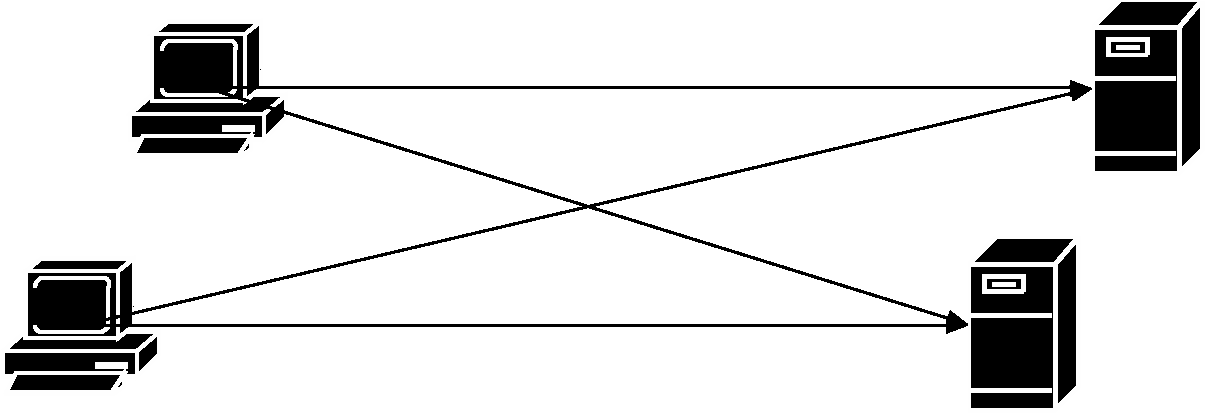
\includegraphics[width=1\textwidth]{graph-lay4}
\end{figure}

\begin{figure}[h]
	\caption{A network observed on the network layer; all devices are interconnected via routers}
	\label{fig:graph-lay3}
	\centering
		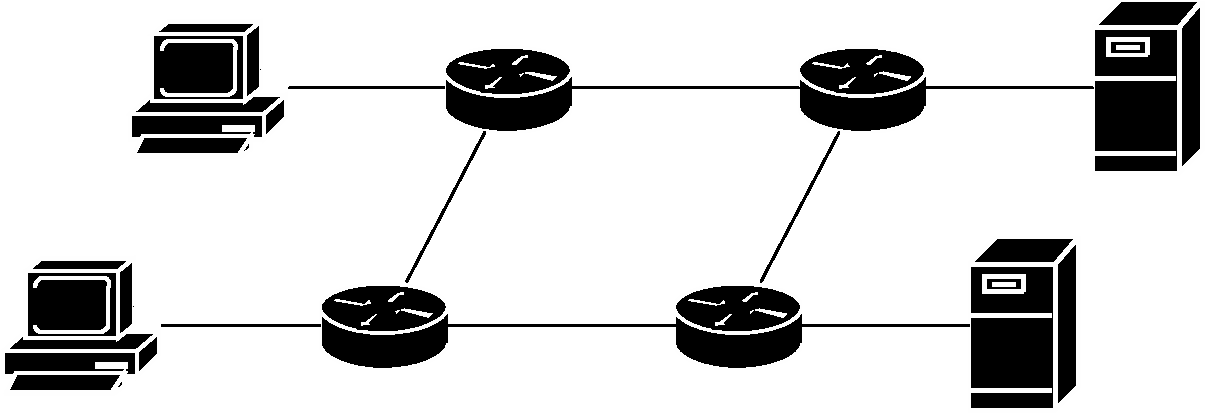
\includegraphics[width=1\textwidth]{graph-lay3}
\end{figure}

The network layer describes how datagrams are routed between two hosts on the network.
This delivery is realised by routers between these hosts,
 where each router forwards datagrams to a router that is closer to the destination.
Datagrams are data packets, which start with an IP-header,
 which contains the source and destination IP address of the datagram.
IP-addresses are fixed-length numbers of 32-bits (IPv4) or 128-bits (IPv6).

The transport layer describes segments being sent directly between hosts,
 not considering any routers.
Typically, segments will have a protocol header, often TCP or UDP.
The TCP and UDP headers contain two 16-bit port numbers (source port and destination port),
which often indicate the kind of traffic in the packet.
For example,
 port 80 indicates web traffic,
 443 indicates encrypted web traffic,
 53 indicates DNS traffic and 22 indicates SSH traffic.


\section{Model optimisation}
\label{sec:model_optimisation}

A possible approach to implement the NetFlow data model as a graph, is to represent IP addresses as vertices, and a combination of (1) ports and (2) time as edges (figure~\ref{fig:graph-pragma}).
This model contains vertices with many edges, which could take a long time to calculate per superstep.
However, this model contains information that is not going to be used.
Removing this information will allow computation to speed up, as unnecessary information will not take up computation time.
In SpreadRank, the \emph{\gls{ephemeral port} number} is not important,
 so it can be discarded.
Because SpreadRank will only look for \gls{spreading} over identical port numbers (using port numbers as a metric for same-type communication),
 the vertices can be split.
The result is a model in which a client that requests a DNS record and then a website will be represented by two vertices;
 one for the DNS client and one for the HTTP client.
The model is inaccurate when compared to real-world TCP or UDP, in that the source port and the destination port are equal
 (whereas in the real world the connections initiated from the client would be initiated from an \gls{ephemeral port}),
 but this model will make it easier to detect \gls{spreading} over identical ports, as will be explained in chapter~\ref{chp:spreadrank}.

\begin{figure}[h]
	\caption{Graph with IP as vertex, ports and time as edge}
	\label{fig:graph-pragma}
	\centering
		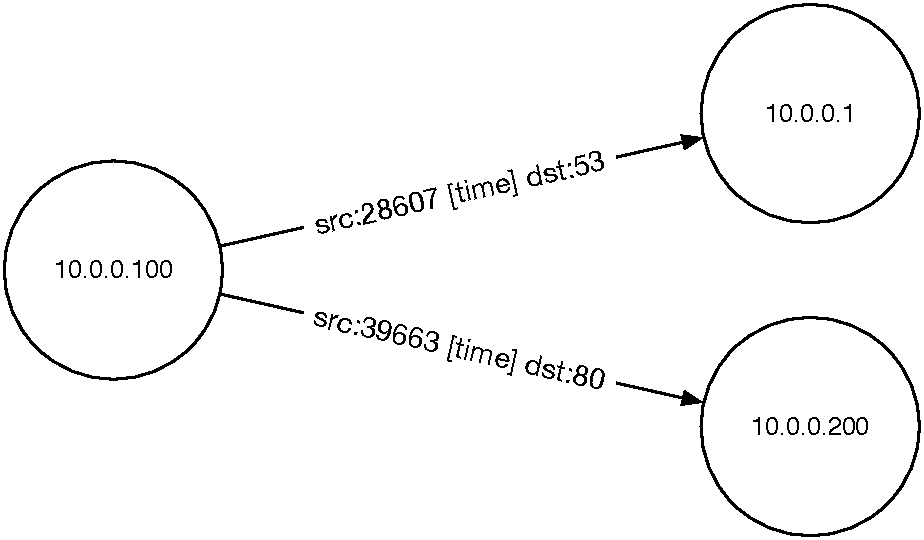
\includegraphics[width=.75\textwidth]{graph-pragma}
\end{figure}

Figure~\ref{fig:graph-optim} shows the optimised version of figure~\ref{fig:graph-pragma}.
There will not be any edge from a DNS vertex to a HTTP vertex.
This will make it easier for Giraph to distribute the graph over different workers,
 in such a way that no vertices need to be moved in between supersteps.

\begin{figure}[h]
	\caption{Graph with IP and port as vertex, time as edge}
	\label{fig:graph-optim}
	\centering
		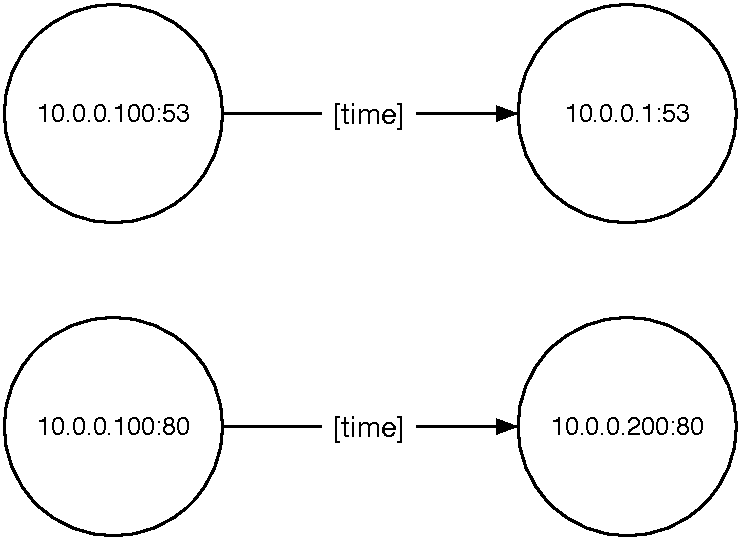
\includegraphics[width=.6\textwidth]{graph-optim}
\end{figure}


\subsection{Data conversion}
\label{sec:conversion}
In order to convert NetFlow to a graph in Giraph,
 an \verb"InputFormat" for NetFlow data must be devised.
Giraph has standard abstract readers and writers available that work with text formats.
For easier implementation, a \gls{bash} script was created that uses \verb"nfdump" to convert NetFlow to \gls{csv} files,
 and a Giraph \verb"EdgeInputFormat" was implemented that reads these \gls{csv} files.

The script filters its output so that only TCP and UDP flows remain where at least one port number is under 1024.
It will invert flows where the source port is the lowest port.
The script passes all its arguments to \verb"nfdump".

The recommended way to use this script is to convert NetFlow logs by day,
 so that multiple Giraph workers can read the graph at the same time.
This will not only speed up reading, but it may prevent a worker crashing from reading a too large file, since the graph is stored in memory.

Using \verb"nfdump" is not ideal, a better solution would have been to use a \verb"NetFlowInputReader" in Giraph directly.
At the time of writing, such a reader was not available.
It is beyond the scope of this thesis to write such an input format reader.

\begin{landscape}
\begin{verbatim}
	#!/bin/bash
	nfdump "$@" -o 'fmt:%ts %te %sa %da %pr %sp %dp %sas %das %in %out %tos %flg' | while read \
	    flowstartdate \
	    flowstarttime \
	    flowenddate \
	    flowendtime \
	    srcaddr \
	    dstaddr \
	    proto \
	    srcpt \
	    dstpt \
	    REST
	do
	    if [ "${proto}" = "TCP" -o "${proto}" = "UDP" ]
	    then
	        if [ "$srcpt" -lt 1024 -a "$dstpt" -ge 1024  -o  "$srcpt" -ge 1024 -a "$dstpt" -lt 1024 ]
	        then
	            [ $srcpt -lt $dstpt ] \
	                && echo $flowstartdate\ $flowstarttime,$dstaddr,$srcaddr,$srcpt \\
	                || echo $flowstartdate\ $flowstarttime,$srcaddr,$dstaddr,$dstpt \\

	        fi
	    fi
	done
\end{verbatim}
\end{landscape}


\section{Spreading}
Most hosts on the internet are either configured as a client or as a server, but some hosts are configured as both.
A server is, for the purpose of this analysis, defined as a host that will receive connections.
A client is, for the purpose of this analysis, defined as a host that will initiate connections.
A connection is thus always initiated by a client, but it allows two-way communication, which allows client and server to exchange information.

This model is based on the assumption that most home users (``clients'') will not run permanent services on their machines,
 but they will use e-mail and browse the web, which they do by contacting servers.
In some cases, however, home users may choose to run servers on their own equipment as well.
This can, for example, be a cheap solution to host a website or a mail server, or it can be done out of curiosity.
On the other hand, servers may themselves be clients, either temporary, for example during maintenance, or as mode of operation, for example a slave DNS server.

In some cases when a client initiates a connection to a server,
 the server may relay this connection to another server, or it may open a similar connection to another server.
This happens for example for proxy servers, which are configured to simply relay information.
Another example is a DNS resolver, which may be queried for a record in the global domain name system.
If it does not have this record available, it will query an authoritative server.

Spreading may also indicate the spreading of malware, for example a computer worm~\cite{pastor2001epidemic}.
By looking at how far traffic spreads and which port number it uses,
 it is possible to get an insight of what happens in the network.
This may prove helpful for finding infected machines in the network.

